\documentclass[10pt,a4paper,twocolumn,twoside]{article}
\usepackage[utf8]{inputenc}
\usepackage[catalan]{babel}
\usepackage{multicol}
\usepackage{graphicx}
\usepackage{fancyhdr}
\usepackage{times}
\usepackage{titlesec}
\usepackage{multirow}
\usepackage{lettrine}
\usepackage[top=2cm, bottom=1.5cm, left=2cm, right=2cm]{geometry}
\usepackage[figurename=Fig.,tablename=TAULA]{caption}
\captionsetup[table]{textfont=sc}

\author{\LARGE\sffamily Christian Espinosa Reboredo}
\title{\Huge{\sffamily Recognition of cognitive states from EEG data}}
\date{}

\newcommand\blfootnote[1]{%
  \begingroup
  \renewcommand\thefootnote{}\footnote{#1}%
  \addtocounter{footnote}{-1}%
  \endgroup
}

%
%\large\bfseries\sffamily
\titleformat{\section}
{\large\sffamily\scshape\bfseries}
{\textbf{\thesection}}{1em}{}

\begin{document}

\fancyhead[LO]{\scriptsize AUTOR: TÍTOL DEL TREBALL}
\fancyhead[RO]{\thepage}
\fancyhead[LE]{\thepage}
\fancyhead[RE]{\scriptsize EE/UAB TFG INFORMÀTICA: TÍTOL (ABREUJAT SI ÉS MOLT LLARG)}

\fancyfoot[CO,CE]{}

\fancypagestyle{primerapagina}
{
   \fancyhf{}
   \fancyhead[L]{\scriptsize TFG EN ENGINYERIA INFORMÀTICA, ESCOLA D'ENGINYERIA (EE), UNIVERSITAT AUTÒNOMA DE BARCELONA (UAB)}
   \fancyfoot[C]{\scriptsize ``Mes'' de 20xx, Escola d'Enginyeria (UAB)}
}

%\lhead{\thepage}
%\chead{}
%\rhead{\tiny EE/UAB TFG INFORMÀTICA: TÍTOL (ABREUJAT SI ÉS MOLT LLARG)}
%\lhead{ EE/UAB \thepage}
%\lfoot{}
%\cfoot{\tiny{February 2015, Escola d'Enginyeria (UAB)}}
%\rfoot{}
\renewcommand{\headrulewidth}{0pt}
\renewcommand{\footrulewidth}{0pt}
\pagestyle{fancy}

%\thispagestyle{myheadings}
\twocolumn[\begin{@twocolumnfalse}

%\vspace*{-1cm}{\scriptsize TFG EN ENGINYERIA INFORMÀTICA, ESCOLA D'ENGINYERIA (EE), UNIVERSITAT AUTÒNOMA DE BARCELONA (UAB)}

\maketitle

\thispagestyle{primerapagina}
%\twocolumn[\begin{@twocolumnfalse}
%\maketitle
%\begin{abstract}
\begin{center}
\parbox{0.915\textwidth}
{\sffamily
%\textbf{Resum--}

%\end{abstract}
%\bigskip
%\begin{abstract}
%\bigskip
%\\
\textbf{Abstract--}An electroencephalogram (EEG) is a test that detects electrical activity of the brain. Since 
1924 this procedure has been done countless times to obtain brain activity. This paper tries to go a step further 
to understand electroencephalography better using deep learning algorithms. The data used in this paper is a public 
dataset CHB-MIT of recordings of paediatric subjects with intractable seizures. Different methods of data management 
are done and documented to make the most of the algorithms used. The objective is to train an algorithm to acknowledge 
when the subject is having a seizure.
\\
\\
\textbf{Keywords-- }electroencephalogram, deep learning, brain activity, classification, EEG analysis\\
}

\bigskip

{\vrule depth 0pt height 0.5pt width 4cm\hspace{7.5pt}%
\raisebox{-3.5pt}{\fontfamily{pzd}\fontencoding{U}\fontseries{m}\fontshape{n}\fontsize{11}{12}\selectfont\char70}%
\hspace{7.5pt}\vrule depth 0pt height 0.5pt width 4cm\relax}

\end{center}

\bigskip
%\end{abstract}
\end{@twocolumnfalse}]

\blfootnote{$\bullet$ E-mail de contacte: christian.espinosar@uab.cat}
\blfootnote{$\bullet$ Menció realitzada: Computació }
\blfootnote{$\bullet$ Treball tutoritzat per: Aura Hernández Sabaté (Ciencies de la Computació)}
\blfootnote{$\bullet$ Curs 2021/22}

\section{Introduction}

\lettrine[lines=3]{A}{n} epileptic seizure is a period of symptoms due to abnormally excessive or synchronous neuronal activity in the brain. This can cause different effects like uncontrolled shaking movements involving much of the body, parts of the body or subtle momentary loss of awareness. In order to understand this issue, it is important to understand how neurons work and interact with each other to conserve what we call consciousness represented as brain activity and brainwaves. 
\\
Neural oscillations are rhythmic or repetitive patterns of neural activity in the central nervous system which can be driven by mechanisms within individual neurons or by interactions. Since 1824 neural oscillations have been observed, fifty years later intrinsic oscillatory behaviour was encountered in vertebrate neurons, but the purpose of these is yet to be fully understood.
\\
In order to understand better brain activity in this TFG tries to dig deeper using new technology like deep learning to try to understand what humans are incapable of doing. First of all, it will be needed an inside view on how the brain works to have a hint on how to extract or intercept information from the neurons to process externally in a computer as well as a view on how deep learning algorithm’s function and get results from data, because it’s the best way to process and get the most out of it. Afterwards an insight of previous papers is given to set a view point on how research has been made up until this point. A well-known database (CHB-MIT) is introduced of encephalograms collected from 23 subject with interactable seizures that has been used in previous research.
\\
Once everything is acknowledged objectives of in this TFG are settled for further research on this issue. First of all, data planning and different treatment procedures are important to see how algorithms behave giving better or worse results, as well as which algorithm architectures are better to process EEG data. Finally, once all the research is done the classifier is to be expected to classify moments where seizures occur on the patients in a given moment.
\\

\section{Brain}
\label{sec-brain}
\subsection{Neuron and neural activity}
\label{subsec-neuron}

To further understand how brain activity works we first need to study a single neuron and its purpose. A neuron is an electrically excitable cell that has the function to communicate with other cells. It does it by nearly touching other cells called synapsis, transmits the message through its axon and delivers the message by synapsis to another cell. Neurons are typically classified into types based on their function:
\\
\begin{itemize}
  \item Sensory neurons: Which respond to stimuli of the sensory organs and send the signals to the spinal cord or brain.
  \item Motor neurons: Its axons originate in the brain and spinal cord and innervate the muscles to produce muscle movements.
  \item Projection fiber: Are neurons found in the central nervous system and only establish synapses with other neurons, these consist of efferent and afferent fibers uniting the cortex with the lower parts of the brain and with the spinal cord.
  \item Interneuron: Is a neuron of the central nervous system, usually small and with a short axon, that interconnects with other neurons, but never with sensory receptors or muscle fibres, allowing it to perform more complex functions.
\end{itemize}
\leavevmode\\
Neurons transmit electrical waves originating from a transient change of permeability in the plasma membrane. Their propagation is due to the existence of a potential difference that arises due to different concentrations of ions on either side of the membrane, as described by the Nernst potential, between the inner and outer part of the cell (typically -70 mV). For the transmission of nervous impulses to other neurons, these do it by synapse, being a structure to pass electrical or chemical signals to another neuron or effector cell, there are two types of synapses:
\\
\begin{itemize}
  \item	Chemical synapse: Electrical activity in the presynaptic neuron is converted into the release of a neurotransmitter that binds to the receptors located in the plasma membrane of the postsynaptic cell.
  \item	Electrical synapse: Is one in which transmission between the first neuron and the second is not by the secretion of a neurotransmitter, but by the passage of ions from one cell to another through gap junctions, small channels formed by the coupling of protein complexes, based on connexins, in closely adherent cells.
\end{itemize}

\leavevmode\\
These electrochemical processes when large numbers of neurons show synchronized activity, electric fields that they generate can be large enough to be detected outside the skull, and so using electroencephalography (EEG) or magnetoencephalography (MEG) brain activity can be recorded.
\\

\subsection{Structure}
\label{subsec-structure}
\leavevmode\\
Now that we know where brain activity originates from, we can further study how the brain structures. There are many parts in the brain, but for now we are going to focus on the cerebrum because it initiates and coordinates movement, regulates temperatures, speech, judgement, reasoning, problem-solving, emotions, learning…
\\
The cerebrum, it’s the largest part of the brain, it’s divided by the medial longitudinal fissure in two hemispheres, each of these hemispheres has an outer layer of grey matter, the cerebral cortex and an inner layer of white matter. The fact that these are separated gives the opportunity for lateralisation of brain functions, which is the tendency of neurological functions to specialise in one hemisphere or the other, but even though the cerebrum is separated, these are connected by the corpus callosum.
\\
The cortex is mapped into fifty different functional areas known as Brodmann’s areas, defined by its cytoarchitecture (cellular composition), or histological structure and organization of cells. One scheme widely used (from Korbinian Brodmann) splits the cortex into 52 different numbered areas of different cellular structure and different functions.
\\
Having clarified this brain structure, obtaining data with electrodes from brain activity, positioning of these is something to keep in touch with depending on what it’s being studied. The same goes for defining the dataset train and test data, to feed as input to the deep learning algorithm, opening a new field on how to treat and subdivide data to make the most of it.
\\

\section{Related Work}
\label{sec-related-work}
A lot of research has been made of the brain to further understand it’s capabilities using deep learning algorithms. Below are different projects attempting to interpret and process EEG data in order to define a baseline of what has been done so far. 
\\
\subsection{Mental Workload Detection based on EEG Analysis}
\label{subsec-work1}
A study of mental workload is done in order to work more efficiently, healthier and to avoid accidents since workload compromises both performance and awareness. The use of EEG signals has a high correlation with specific cognitive and mental states such as workload, proposing a binary neural network to classify EEG features across different mental workloads.
\\
Mental workload is defined as “the cognitive and psychological effort to conclude a task”, observing that depending if workload is too heavy or too light this can affect human performance. Also, since workload involves neuro-physiologic, and perceptual processes it is affected by individual capabilities, motivation to preform, physical and emotional state which it’s multifaceted nature of workload prevents it of studying directly but it is feasible to infer this from a number of quantifiable variables.
\\
There are two main categories to measure workload:
\\
\begin{itemize}
\item Subjective measures: Being the most used to asses mental workload, the NASA Task Load Index (TLX) a prominent way to gain insight on perceived workload from the subject based on a weighted average of six sub-variables: mental demand, physical demand, temporal demand, performance, effort and frustration. Widely used in aviation to assess mental workload of the pilot but it is highly subjective.
\item Physiological measures: Providing a more reliable data by measuring physiological dynamic changes which cannot be controlled consciously, so that is why it’s more reliable. Readings such as electrocardiogram (ECG), electromyograph, electroencephalogram (EEG), photoplethysmography, respiration rate sensors, electro-dermal activity (EDA), oxygen density in the blood in the brain, and eye movement trackers... The combination of inputs reports better accuracy than the analysis if each one independently.
\end{itemize}
\leavevmode\\
The approach is to investigate the ability of 1D-CNN models to recognise two types of mental load from EEG signals and to generalise the model to a population not seen in the training set. They use N-back test (memory demanding games requiring the resolution of simple arithmetic operations adjusting workload) to induce low and medium workload and to classify a simple neural network (NN) it’s trained using only the power spectrum of theta waves. Proposing a personalized model for each individual and a generalist one, preform the models in a dataset of 16 subjects showing outstanding results in a leave-one-out subject test and so generalizing to new unseen subjects.
\\
The method to obtain data all 16 subjects had to first watch a 10-minute relaxing video and afterwards do the N-back-test low, medium and high difficulty. Finally subjects ask a TLX questionnaire for subjective perception of the test difficulty and workload.
\\
To get the data itself EEG recordings were done using EMOTIV EPOC+ headset which has 14 electrodes placed according to the 10/20 system which provide raw data and power spectrum for the main brain rhythms (theta, alpha, beta low, beta high, and), at 128 Hz and 8 Hz, respectively. Data had to be filtered from noise with Inter Quartile Range (IQR) strategy to detect outlier values associated to muscular movement wave peaks. In this work, power spectrum used was from theta wave (4-8Hz) sampled at 8Hz feed into the models in 5 second windows of every electrode (14 EEG sensors). Variables were normalized to have 0 mean and
sigma=1 using the mean and standard deviation of the training set. 
\\
Networks have a hidden layer of 128 neurons with ReLU as the activation function. Before the classification layer a dropout layer was added to avoid overfitting and all models have been trained using weighted cross-entropy loss, to compensate the different lengths of base line and workload phases which introduces unbalance in data samples.
\\
In conclusion its reported 95\% confidence interval for each class computed for all subjects and recall above 90\%. It is suggested to use longer windows to capture EEG non stationary nature.
\\
%\subsection{EEG SIGNAL DIMENSIONALITY REDUCTION AND CLASSIFICATION USING TENSOR DECOMPOSITION AND DEEP CONVOLUTIONAL NEURAL NETWORKS}
%\label{subsec-work2}


\section{Objectives}
\label{sec-objectives}
There are two main objectives in this TFG. The first objective is to find the best way to treat, analyse and classify data before feeding it to the deep learning algorithms, for example, as a continuous stream of sequence, dividing data per subject…  or trying different test/train strategies such as leave one out, 50/50… The second main objective is to try to find which algorithms architectures have better results with the data, for example CNN, Transformer, SVM…
\\

\section{Tasks}
\label{sec-tasks}
To start from somewhere the first task will be to use an already done deep learning algorithm from the research group IAM from the CVC, which is working on a framework to determine the optimal architecture for cognitive state recognition from EEG signals, with the objective to answer different questions:
\begin{itemize}
  \item How to combine the signals to create the input features for feature extraction? In this case, having 14 sensors x 5 waves, so 70 raw signals. These signals can be concatenated, or projected. As well, in case of projection, the weights can be equal or learned.
  \item Which neural network is the best performer?
  \item Is it better to ensemble the different classifiers before combining the signals?
\end{itemize}
\leavevmode\\
This framework was originally intended to study brain workload, so, within this framework, the idea is to modify it to fulfil the objective of clinic seizure detection. In this TFG, different strategies will be applied on the input data of the algorithm to further study it’s capabilities.
\\
If this itself it’s already done within the period of completion of this research and there is still time for more tasks, a new neural network will be created. A deep search on what architectures there are, and which suits better for this work will be done and a new model will be created from scratch. Afterword the models will be compared and reported to learn which preform better in different conditions.
\\
Diferent tasks to be done:
\begin{figure}[!h]
  \centering
    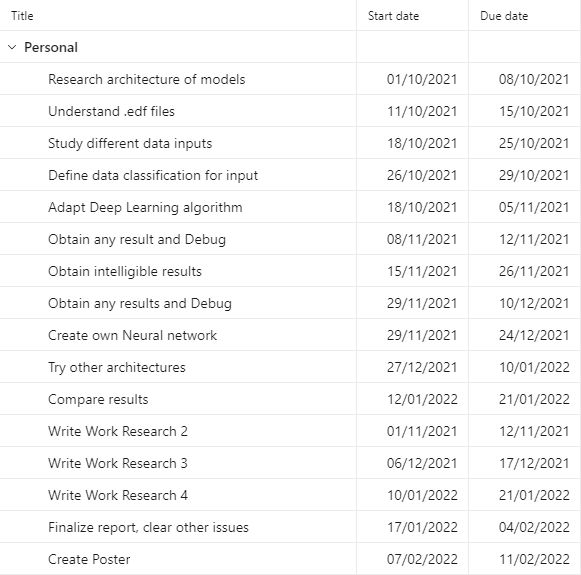
\includegraphics[width=0.4\textwidth]{img/Tasks.png}
    \caption{General Tasks of the TFG}
    \label{fig-exemple}
  \end{figure}

Note that “Write Work Reaserch” tasks are before every meeting.
\leavevmode\\

\begin{figure*}[!h]
  \centering
    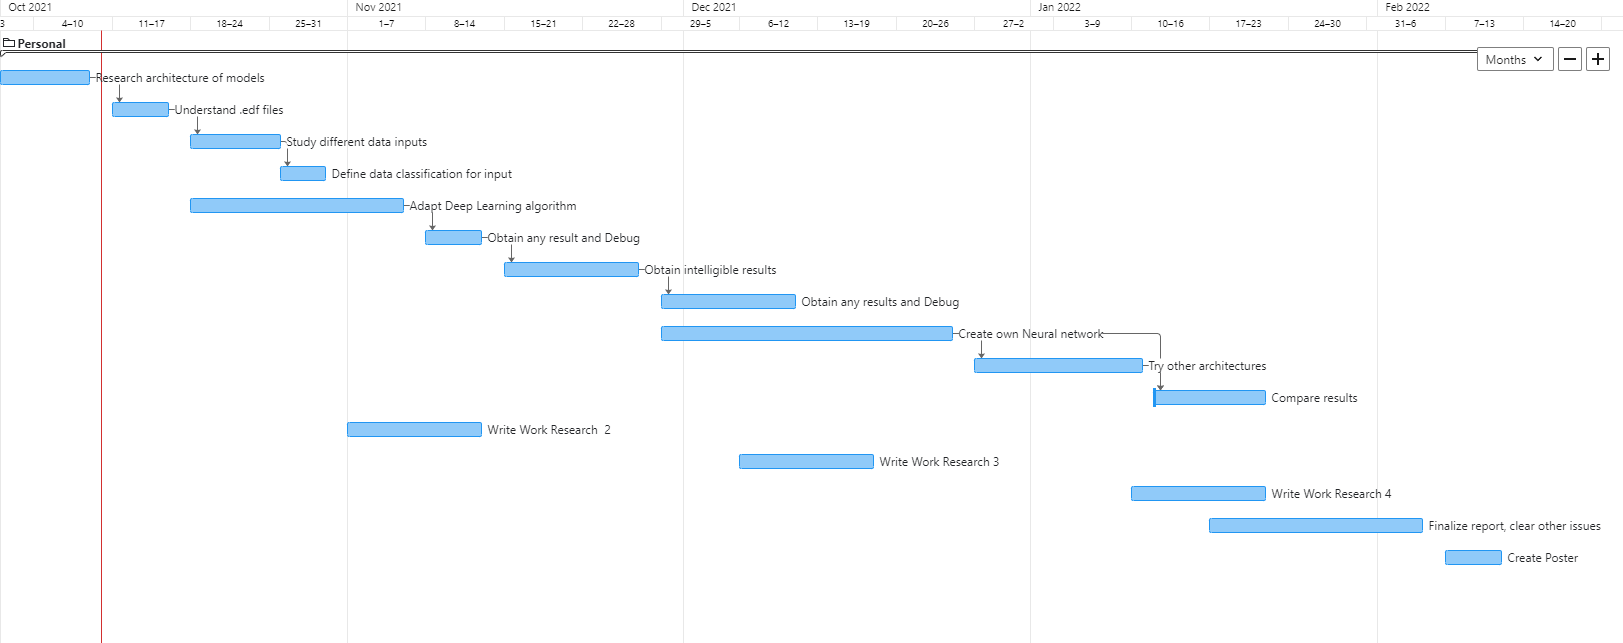
\includegraphics[width=1\textwidth]{img/Gantt.png}
    \caption{Gantt Diagram of the project}
    \label{fig-exemple}
  \end{figure*}

%\section*{Agraïments}

%\begin{thebibliography}{11}

%\bibitem{neural_oscilation}
%https://en.wikipedia.org/wiki/Neural\_oscillation

%\bibitem{seizure}
%https://en.wikipedia.org/wiki/Seizure

%\bibitem{latex}
%http://en.wikibooks.org/wiki/LaTeX

%\bibitem{the}
%http://www.acnweb.org/acta/2002\_18\_2\_104.pdf

%\bibitem{other projects}
%https://arxiv.org/pdf/1908.10432v1.pdf

%\bibitem{dataset}
%https://paperswithcode.com/dataset/chb-mit



%\end{thebibliography}

\end{document}

